\toclesssection{SCP 034 - Obsidian Ritual Knife}
\addcontentsline{toc}{section}{SCP 034 - Obsidian Ritual Knife}

\textbf{Item \#:} SCP-034

\textbf{Object Class:} Euclid

\begin{figure}[h]
\begin{center}
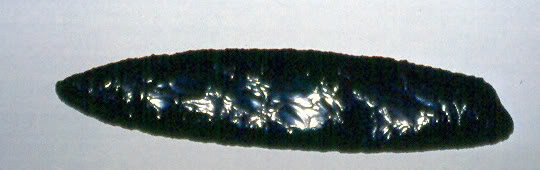
\includegraphics[scale=0.4]{scp/034.jpg}
\linebreak File photo of SCP-034
\end{center}
\end{figure}

\textbf{Special Containment Procedures:} SCP-034 is to be kept in a secure room with access granted only to Level 4 personnel. SCP-034 itself will be kept in a locked case that is under 24-hour surveillance. When not in lab conditions, SCP-034's protective sheath cannot be removed under any circumstances. Any personnel in contact with SCP-034 must be placed under a 24-hour observation period until their identities can be confirmed.

\textbf{Description:} SCP-034 is a primitive knife constructed out of pure obsidian. Tests reveal that SCP-034 is approximately 1000 years old. Despite its crude method of construction and age, SCP-034 is still incredibly sharp and requires no maintenance at all. Expert analysis hypothesizes that SCP-034 may be of South American origin, and that it was used in Native American rituals. Several accounts from Spanish conquistadors exploring the █████████ region support this hypothesis, with detailed writings on how █████ priests would flay their victims alive with similar knives and wear their skin as a tribute to their gods.

SCP-034 has the ability to allow its bearer to take on the appearance of another individual. If SCP-034 is used to cut a piece of flesh from a living individual, and that piece of flesh is placed against the skin of another individual, the second individual would take on not only the appearance, but all physical characteristics of the first individual. Testing has shown that the minimum amount of skin required can be as little as one (1) square centimeter. However, testing has also revealed that the amount of time the facade lasts is directly proportional the amount of flesh used. The ratio of time the facade lasts to flesh used has been measured at approximately one (1) hour for every square centimeter used. Once the time limit has passed, the affected individual will revert to his original form.

Analysis of SCP-034's ability shows that its method of mimicking another individual is nearly flawless. Not only does SCP-034 change physical appearance, but actual physical attributes as well, including height, weight, muscle mass, bone density, hair growth, eyesight, strength, physical medical conditions, and even DNA. Subjects still retain their original personality and memories. Even though the process is nearly instantaneous, taking only a few seconds, human test subjects have described the transformation process as extremely painful. Subjects also may suffer psychological trauma depending on the extent of their physical transformation. Side effects are especially serious if the subject takes on the appearance of a person with differing gender or with wildly different physical attributes.

However, in order to function properly, the individuals who have their flesh cut off by SCP-034 must still be biologically alive to maintain the facade. Should the individual whose identity has been stolen expire, the effect immediately wears off. Further details may be found in Lab Report 034A. Also, SCP-034 only appears to work on human subjects. Cross-species experiments with SCP-034 have resulted in [DATA EXPUNGED]

SCP-034 came into Foundation possession when an imposter disguised as Dr. \censor{XXXXXXX} attempted to infiltrate Site \censor{XX}. The impostor was apprehended when authorities discovered the real Dr. \censor{XXXXXXX} tied up in his home with a large portion of his right arm skinned. Further details may be found in Post Interrogation Report 2211.

\textbf{Lab Report-034A:} \textsl{We've decided to test several scenarios dealing with the limits of SCP-034's capabilities.}
\begin{itemize}
\item Test 1: Sample taken from deceased human cadaver and applied to subject D-452. No effect.

\item Test 2: Sample taken from D-532 and applied to D-452. D-452 successfully mimics D-532's appearance. Upon termination of D-532, D-452 immediately reverts back to original form.

\item Test 3: Sample taken from a brain-dead medical patient and applied to subject D-452. D-452 successfully mimics the patient's appearance and manages to maintain the facade.

\item Test 4: Sample taken from a terminally ill medical patient and applied to subject D-452. D-452 successfully mimics the patient's appearance as well as the patient's illness. Both the terminally ill patient and D-452 expire at the same time, after which D-452 reverts back to original form.

\item Test 5: [DATA EXPUNGED]
\end{itemize}
\newpage
\textbf{Post Interrogation Report 2211:}
\textsl{As per standard operating procedure, we first attempted to interrogate the prisoner via non-violent and non-invasive means. However, when such methods proved ineffective, we began to implement conventional interrogation techniques. While partially successful, we deemed it necessary to use SCP-\censor{XXX}, SCP-\censor{XXX}, SCP-\censor{XXX}, and SCP-\censor{XXX}. We managed to learn the following facts:}
\begin{itemize}
\item \textsl{*The prisoner had extensive knowledge on the existence of the Foundation and its inner workings.}
\item \textsl{The prisoner had extensive knowledge on other SCP-related agencies and groups.}
\item \textsl{The prisoner was not acting under any official capacity from any government agency.}
\item \textsl{The prisoner obtained SCP-034 and instructions on its operation from an unknown benefactor.}
\item \textsl{The prisoner was given very specific instructions to infiltrate Site-\censor{XX} and maintain his position until further notice.}
\item \textsl{The prisoner had enough samples of Dr. \censor{XXXXXXX} to stay within Site-\censor{XX} for \censor{XX} days.}
\end{itemize}
\textsl{Regrettably, the prisoner did not survive interrogation. -Agent \censor{XXXXXX}}
